\documentclass{beamer}
\usetheme{Madrid}
%\usepackage[fontset=mac]{ctex} % 若使用中文则取消注释
\usepackage{ulem}
\usepackage{graphicx}
\usepackage{subcaption}
\usepackage{amsmath}
%\lstset{breaklines}
%\lstset{extendedchars=false}
\usepackage{smartdiagram}          % Provides simple flowchart layouts
\usesmartdiagramlibrary{additions} % Allows extra custom formatting
\usepackage{booktabs} 
\documentclass{article}
\usepackage{tikz}
\usetikzlibrary{positioning, arrows.meta}


\title[Geo-Distributed Training]{
    Train Large Models Across the World
}
\subtitle{Accelerating Training on Geo-Distributed Clusters via Heterogeneity-Aware Collective Communication}
\author{Yuxiang Lin \and Tianjun Yuan}
\institute{\{yl925, ty117\}@duke.edu}
\date{April 2025}
%\titlegraphic{\includegraphics[width=2cm]{logo.png}} % 如果有 Logo，取消注释

\begin{document}

\begin{frame}
  \titlepage
\end{frame}


% Table of Contents Slide
\begin{frame}{Outline}
    \tableofcontents
\end{frame}

% Slide 1: Brief Introduction
\section{Background and Introduction}
\begin{frame}
  \frametitle{Outline}
  \tableofcontents[currentsection]
\end{frame}

% \begin{frame}{Model Scaling}
%     \centering
%     \begin{tabular}{lcc}
%         \toprule
%         \textbf{Configuration} & \textbf{LLaMA-3-70B} & \textbf{llAma-Our-70000B} \\
%         \midrule
%         Hidden Size & 8,192 & 46,000 \\
%         Transformer Layers & 80 & 256 \\
%         Total Parameters & 70B & 70,000B (70T) \\
%         \bottomrule
%     \end{tabular}

%     \vspace{0.5cm}
%     \small Note: The above scaling does not even consider Mixture-of-Experts (MoE) architectures, which might requires more GPU memory (i.e. deepseek-v3).

% \end{frame}

\begin{frame}{Scaling Models vs Scaling Infrastructure}
    \centering
    \small

    \begin{minipage}{0.48\linewidth}
        \centering
        \textbf{Larger, Deeper Models \\ (e.g. From 405B)} \\
        \vspace{0.5em}
        \begin{tabular}{ll}
            \toprule
            \textbf{Metric} & \textbf{Value} \\
            \midrule
            Hidden Size & 16,000 → 96,000 \\
            Transformer Layers & 128 → 384 \\
            Total Parameters & 405B → 405T \\
            Training Cost & Extremely High \\
            \bottomrule
        \end{tabular}


        \vspace{2.3em}
        \textit{Challenges: stability, compute, memory, training time}
    \end{minipage}
    \hfill
    \vrule width 0.5pt
    \hfill
    \begin{minipage}{0.48\linewidth}
        \centering
        \textbf{Faster, Smarter Networks} \\
        \vspace{0.5em}
        \begin{tabular}{ll}
            \toprule
            \textbf{Aspect} & \textbf{Trend} \\
            \midrule
            Network Scope & Intra-area → Inter-city \\
            Bandwidth & Increases drastically \\
            Latency & Drops significantly \\
            \bottomrule
        \end{tabular}

        \vspace{5.0em}
        \textit{Opportunities: flexibility, scalability, collaboration}
    \end{minipage}
    \vspace{3.0em}
    
    Note: Our simulations are now based on LLaMA-3-405B, while the method remains applicable as the model scales up.
\end{frame}



\begin{frame}{Decentralized Regime Training (Neurips 2022 Oral)}

    
    \begin{figure}
        \centering
        % 调整图片宽度以避免超出页面
        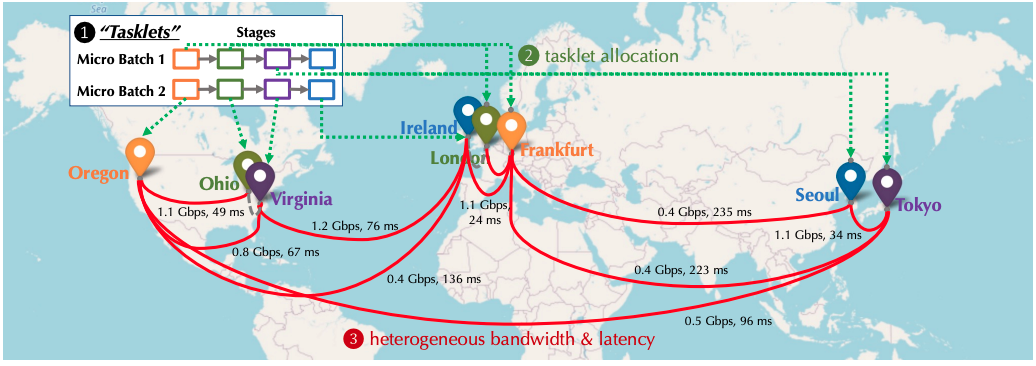
\includegraphics[width=0.9\linewidth]{fig/nips_2022.png}
        \caption{https://openreview.net/pdf?id=UHoGOaGjEq}
    \end{figure}
\end{frame}


\begin{frame}{Decentralized Regime Training}
    \begin{figure}
        \centering
        \begin{minipage}{0.43\linewidth}
            \centering
            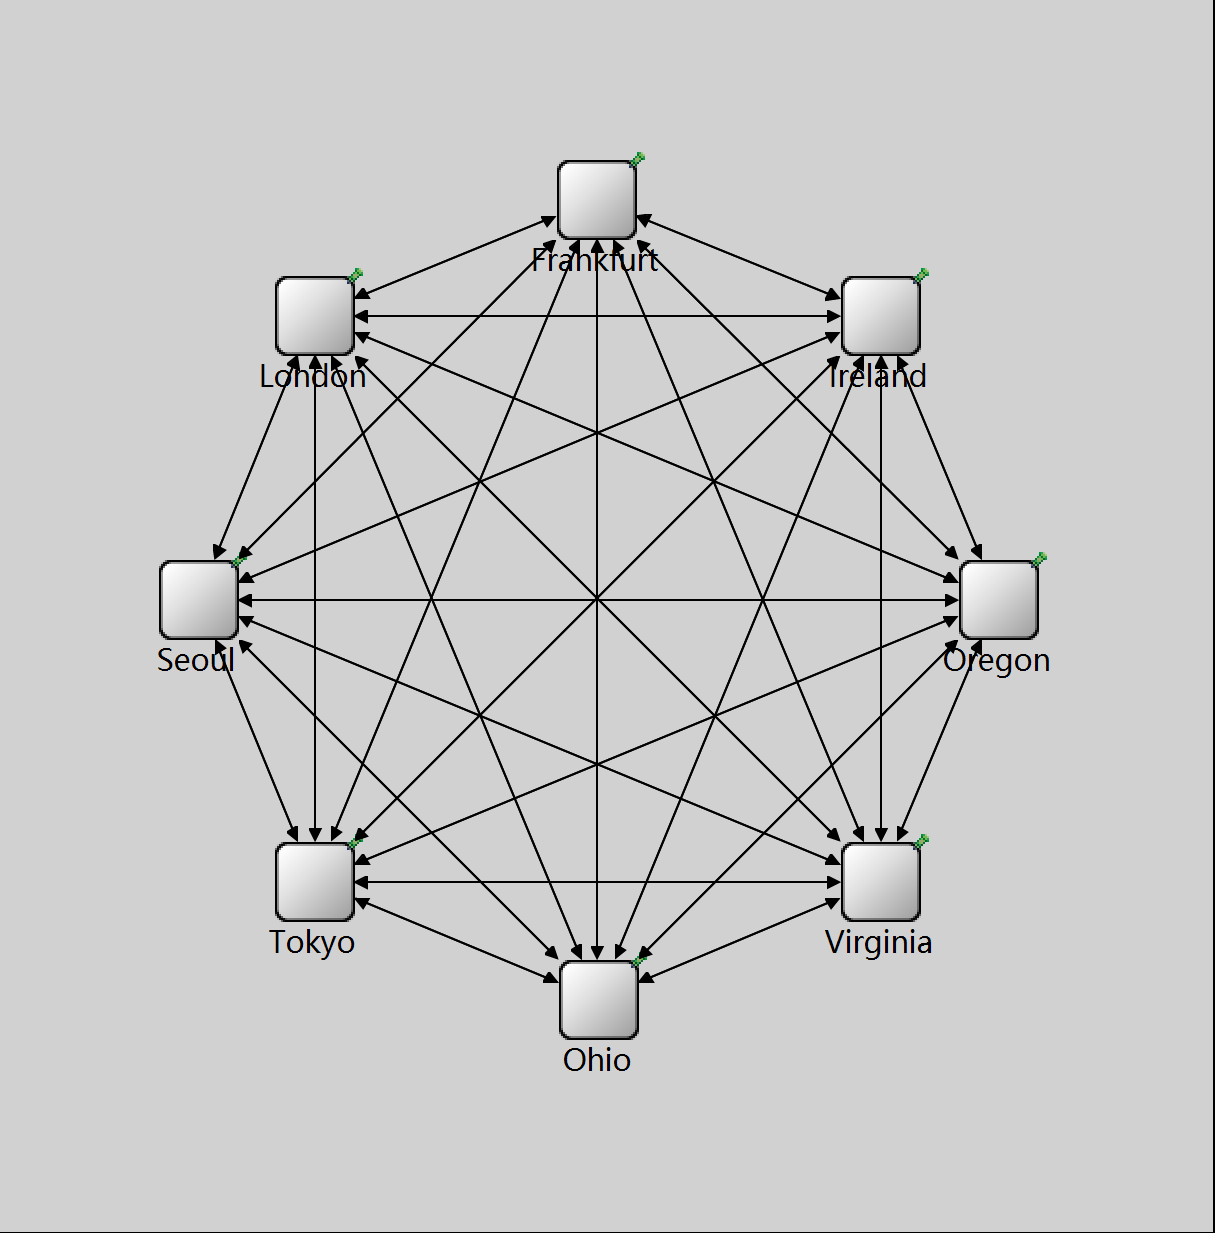
\includegraphics[width=\linewidth]{fig/their_topology.png}
            \caption{Their Topology \\ 
                    (By OMNeT++)}
            \label{fig:their-topology}
        \end{minipage}
        \hfill
        \begin{minipage}{0.55\linewidth}
            \begin{itemize}
                \item Several computation centers might be located in a close area. They might form a clique, with one node dominating.
                \begin{itemize}
                    \item \textcolor{teal}{We propose a new topology to better handle this scenario.}
                \end{itemize}

                \item They applied data parallelism and pipeline parallelism
                \begin{itemize}
                    \item \textcolor{teal}{We added the third: tensor parallelism.}
                \end{itemize}
                
                \item We consider heterogeneous computation resources across clusters.
            \end{itemize}
        \end{minipage}
    \end{figure}
\end{frame}

\section{Proposed Method}
\begin{frame}
  \frametitle{Outline}
  \tableofcontents[currentsection]
\end{frame}

\begin{frame}{Regional Subserver}
    \begin{figure}
        \centering
        \begin{minipage}{0.49\linewidth}
            \centering
            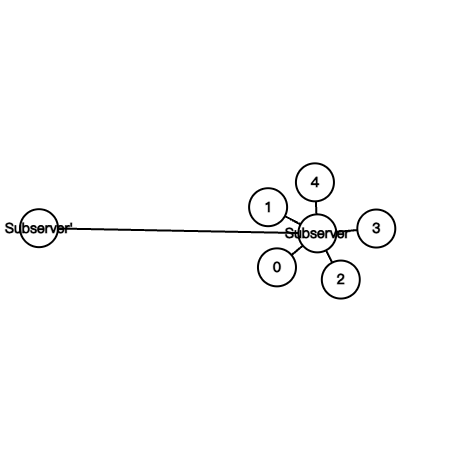
\includegraphics[width=\linewidth]{fig/subserver.png}
            \caption{Introducing Subserver}
            \label{fig:their-topology}
        \end{minipage}
        \hfill
        \begin{minipage}{0.5\linewidth}
            \begin{itemize}
                \item The edges between subserver are be directed; they form a chain.  
                \begin{itemize}
                    \item \textcolor{teal}{This allows us to split the model across subserver.}
                \end{itemize}
                \item Cluster-Subserver Connection: Large bandwidth and small latency
                \begin{itemize}
                    \item \textcolor{teal}{The subserver (with large bandwidth and low average lantency) plays the role of a transit hub for ALLREDUCE.}
                \end{itemize}
                
                \item Inter-Subserver Connection: LARGE bandwidth to support LARGE batch parallel transmitting.
            \end{itemize} 
        \end{minipage}
    \end{figure}
\end{frame}


\begin{frame}{Topology Comparison in OMNeT++}
    \begin{figure}
        \centering
        \begin{minipage}{0.48\linewidth}
            \centering
            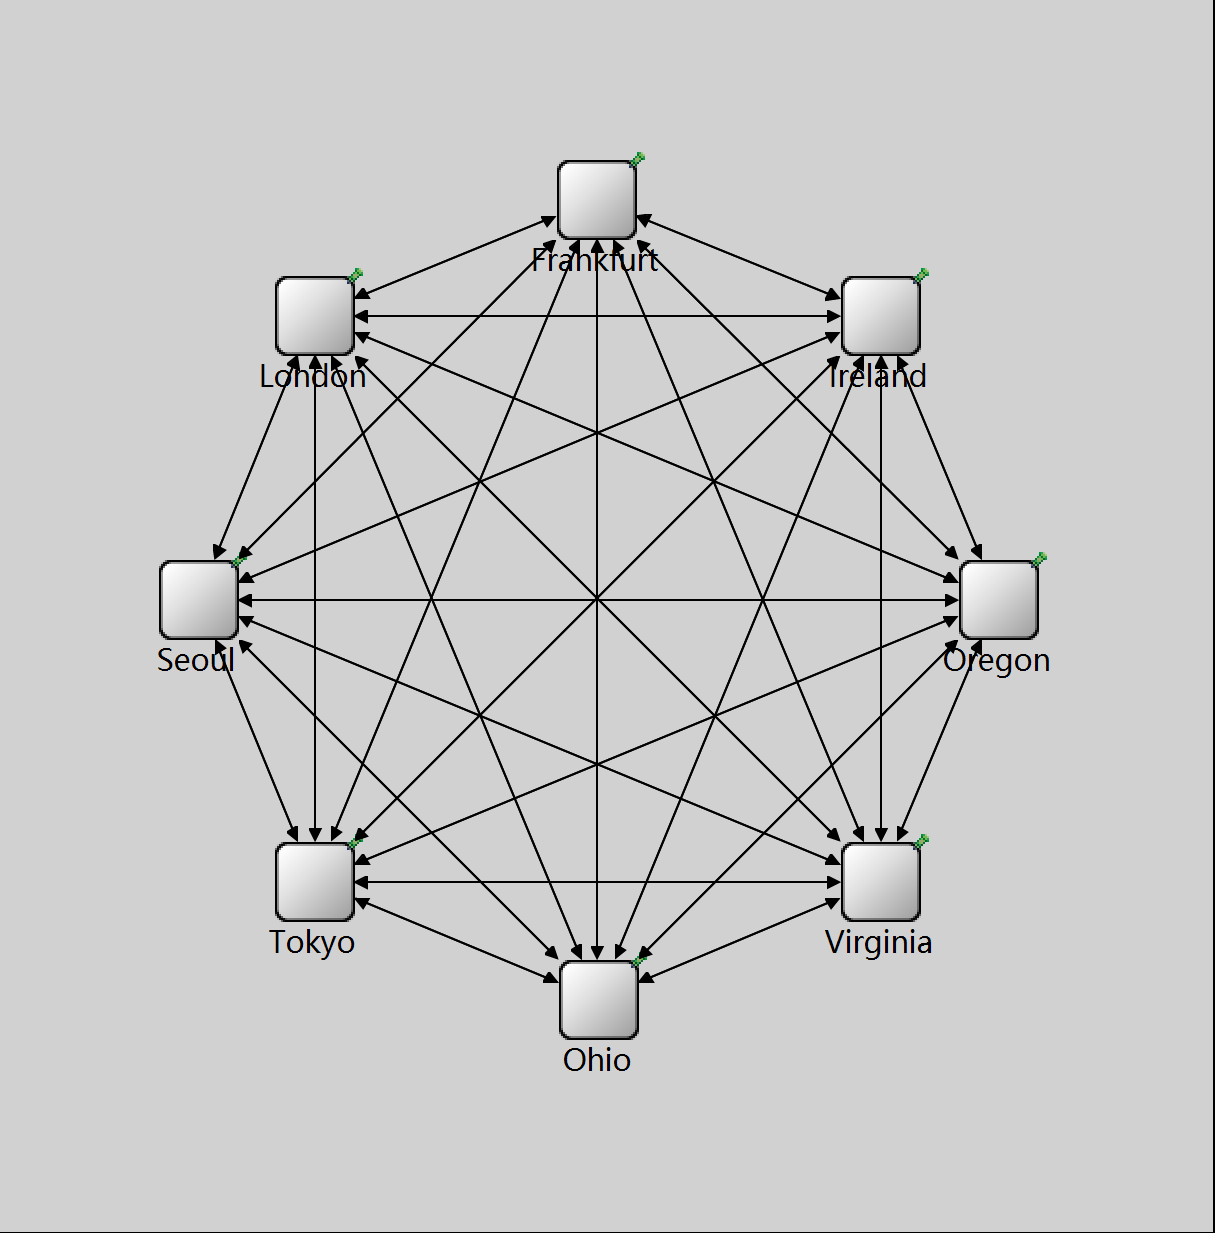
\includegraphics[width=\linewidth]{fig/their_topology.png}
            \caption{Their Topology}
            \label{fig:their-topology}
        \end{minipage}
        \hfill
        \begin{minipage}{0.48\linewidth}
            \centering
            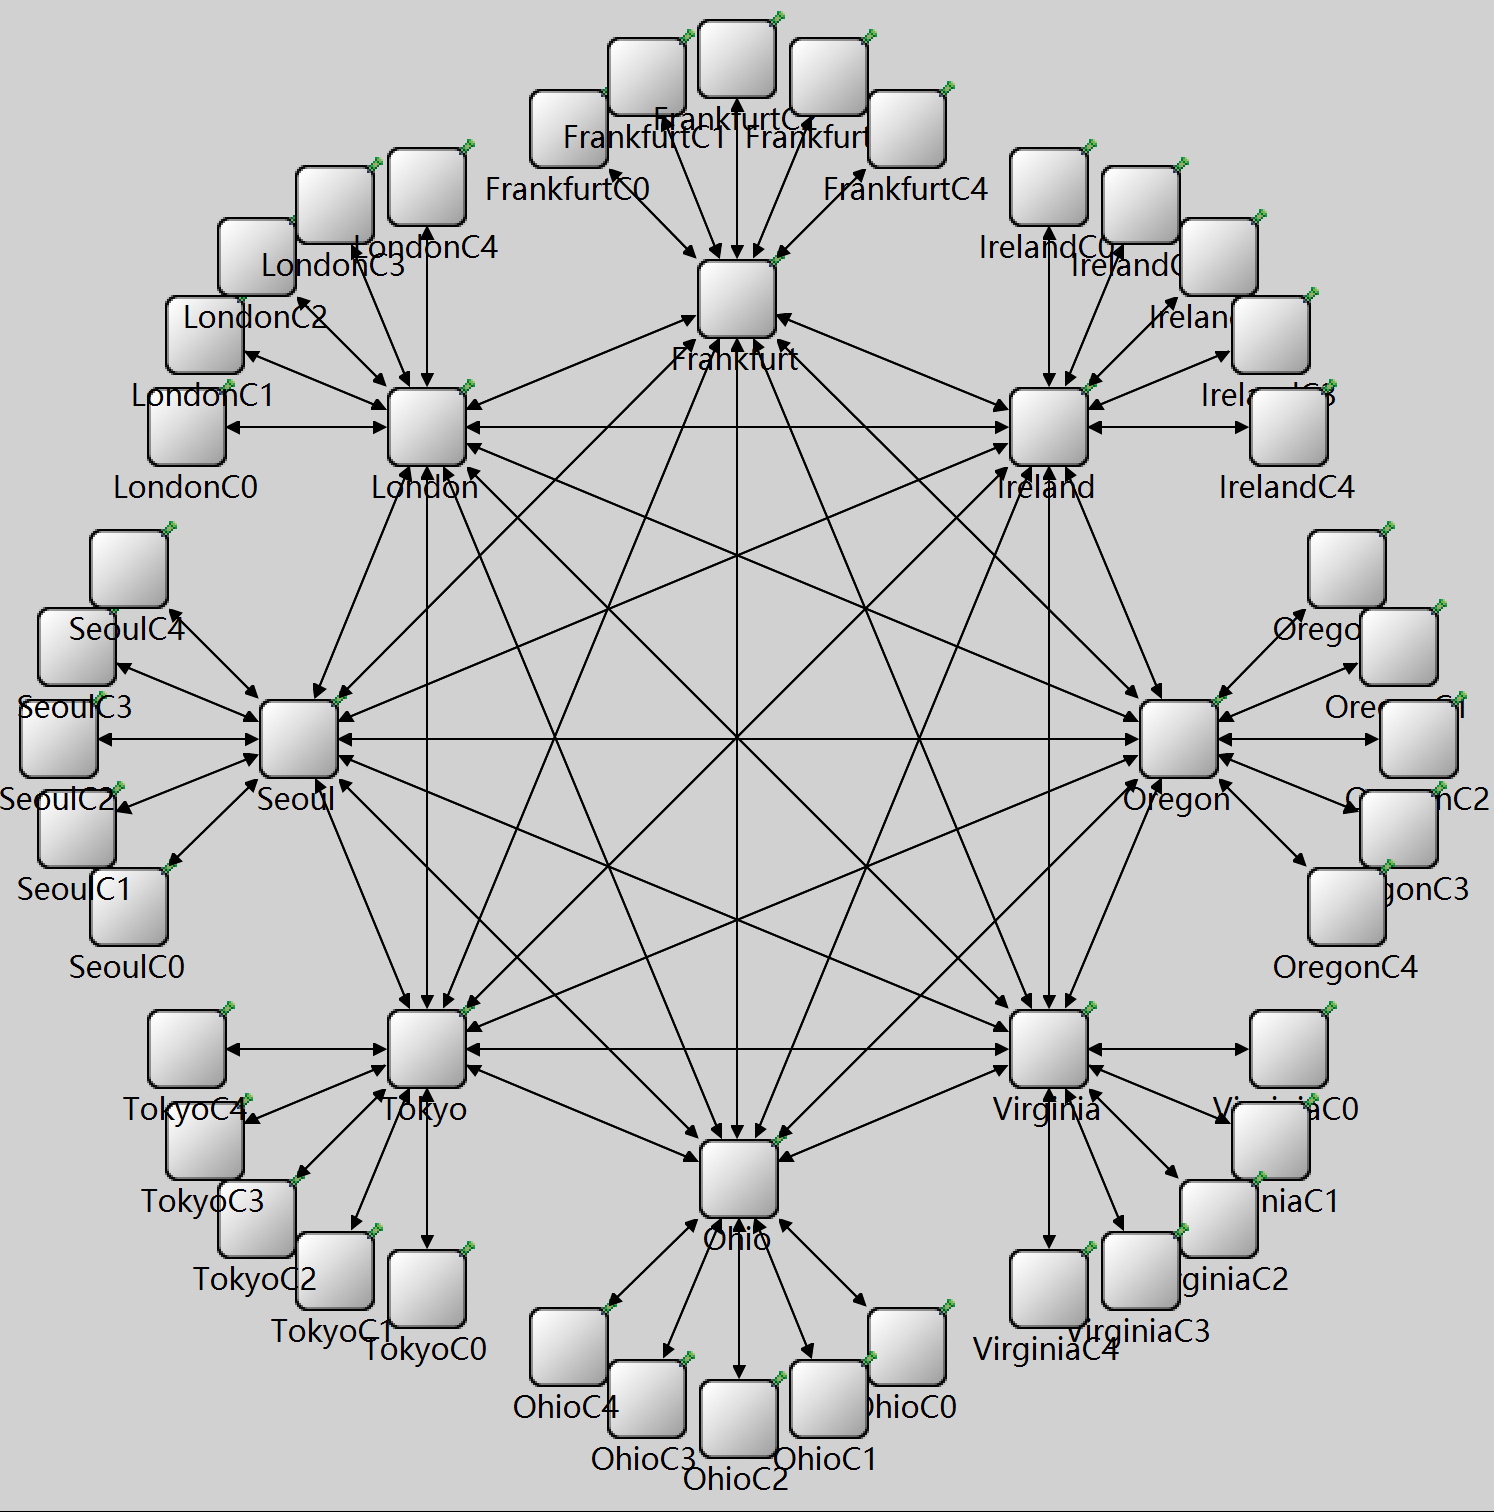
\includegraphics[width=\linewidth]{fig/our_topology.png}
            \caption{Our Topology}
            \label{fig:our-topology}
        \end{minipage}
    \end{figure}
\end{frame}

\begin{frame}{Recap: Parallelism}

    \begin{itemize}
        \item \textbf{Data Parallelism}: The model is replicated across multiple devices, and each device processes a different mini-batch of input data. 
        
        \item \textbf{Pipeline Parallelism}: The model is split into multiple layers, each assigned to a different device.
        
        \item \textbf{\textcolor{blue}{Tensor Parallelism (What they haven't done)}}: Individual model layers are partitioned across devices at the tensor level. Each device computes a slice of the tensor.
    \end{itemize}
\end{frame}

\begin{frame}{A Simple Transformer}

    \begin{figure}
        \centering
        % 调整图片宽度以避免超出页面
        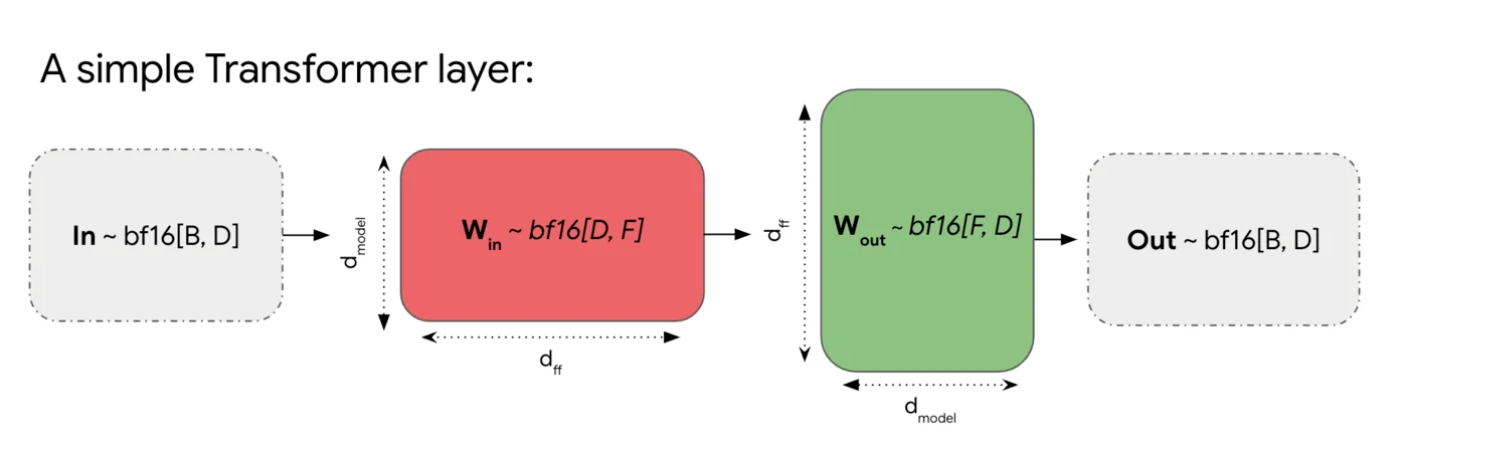
\includegraphics[width=0.9\linewidth]{fig/simple.png}
        \caption{https://jax-ml.github.io/scaling-book/training/#mixed-fsdp-and-tensor-parallelism}
    \end{figure}
\end{frame}


\begin{frame}{Tensor Parallelism}

    \begin{figure}
        \centering
        % 调整图片宽度以避免超出页面
        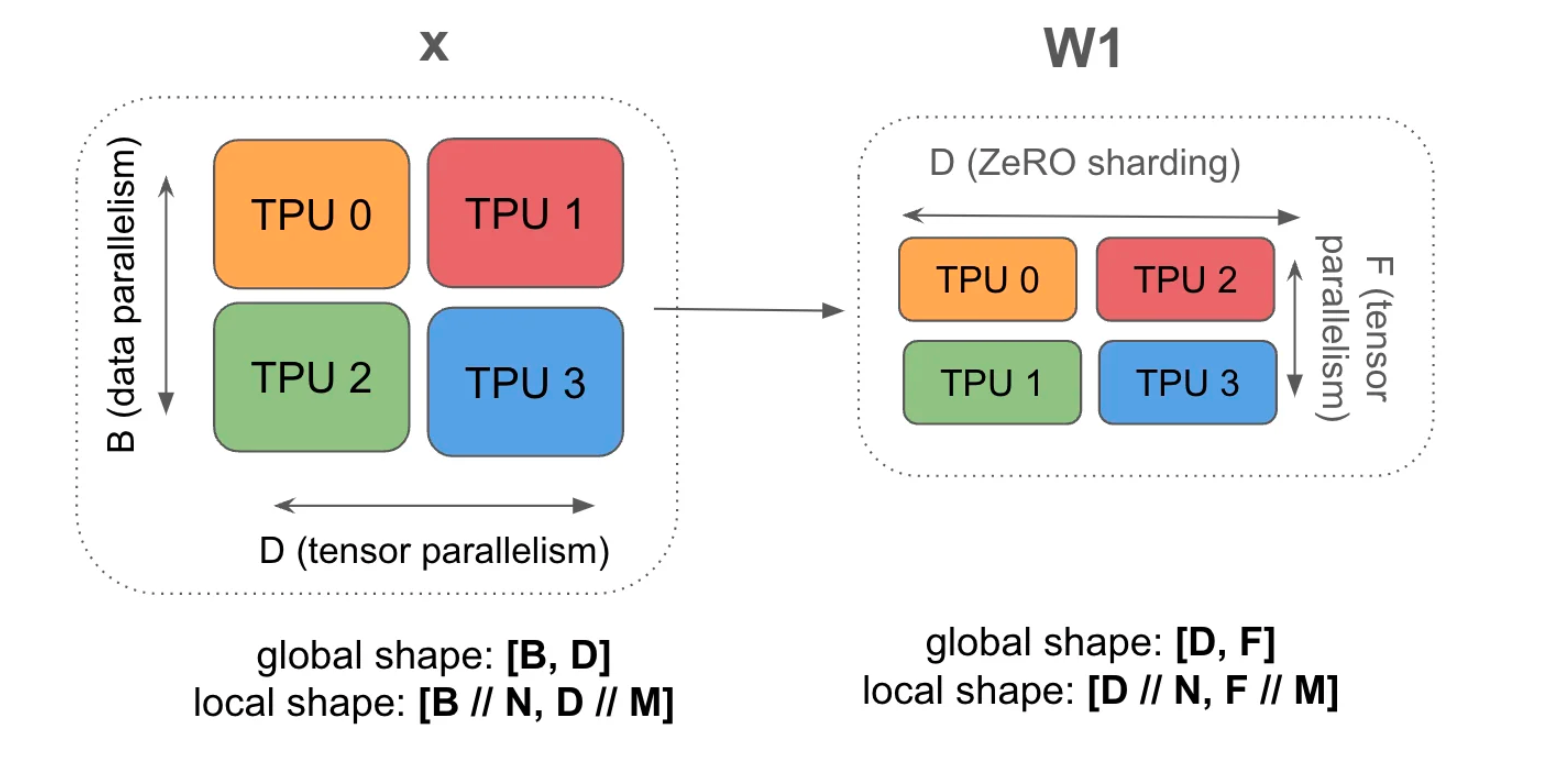
\includegraphics[width=0.9\linewidth]{fig/tensor.png}
        \caption{https://jax-ml.github.io/scaling-book/training/#mixed-fsdp-and-tensor-parallelism}
    \end{figure}
\end{frame}

\section{Training Algorithm Implemented}
\begin{frame}
  \frametitle{Outline}
  \tableofcontents[currentsection]
\end{frame}

\begin{frame}{Pipeline + Data Parallelism}
    Consider having two microbatches in a single batch, and three clusters:
    \vspace{5.0em}
    
    \begin{tabular}{l|l|l|l|l|l|l|l}
        Cluster \textbackslash Time & 0 & 1 & 2 & 3 & 4 & 5 & 6  \\
        \hline
        0 & 0F & 1F & & & 0B & 1B & ReduceAll \\
        \hline
        1 & & 0F & 1F & 0B & 1B & ReduceAll \\
        \hline
        2 & & & 0F & 1F & ReduceAll & &
    \end{tabular}
\end{frame}


% \begin{frame}{Forward Pass Dependency Graph}

% \begin{tikzpicture}[
%   node distance=1.4cm and 2.2cm,
%   box/.style={draw, rounded corners, minimum width=2.8cm, minimum height=1cm, align=center},
%   arrow/.style={->, thick},
%   font=\footnotesize
% ]

% % Top inputs
% \node[box] (in) {In[$B_X$, D]};
% \node[box, right=of in] (win) {$W_{\text{in}}$[D, F]};

% % Combine line for *D
% \node[coordinate, below=0.8cm of in] (mid1l) {};
% \node[coordinate, below=0.8cm of win] (mid1r) {};
% \node[coordinate, below=0.4cm of $(mid1l)!0.5!(mid1r)$] (joinD) {};
% \node[box, below=of joinD] (tmp) {Tmp[$B_X$, F]};

% % From tmp to Out
% \node[box, right=of tmp] (wout) {$W_{\text{out}}$[F, D]};
% \node[coordinate, below=0.8cm of tmp] (mid2l) {};
% \node[coordinate, below=0.8cm of wout] (mid2r) {};
% \node[coordinate, below=0.4cm of $(mid2l)!0.5!(mid2r)$] (joinF) {};
% \node[box, below=of joinF] (out) {Out[$B_X$, D]};
% \node[box, below=of out] (loss) {Loss[$B_X$]};

% % Arrows
% \draw[arrow] (in) -- (mid1l);
% \draw[arrow] (win) -- (mid1r);
% \draw[arrow] (joinD) -- (tmp);
% \node at ($(mid1l)!0.5!(mid1r)+(0,-0.2)$) {*D};

% \draw[arrow] (tmp) -- (mid2l);
% \draw[arrow] (wout) -- (mid2r);
% \draw[arrow] (joinF) -- (out);
% \node at ($(mid2l)!0.5!(mid2r)+(0,-0.2)$) {*F};

% \draw[arrow] (out) -- (loss);

% \end{tikzpicture}

% \end{frame}


\begin{frame}[fragile]{Data Parallel: Forward Pass}

\textbf{Forward Pass} (compute Loss[\texttt{B$\times$1}]):\vspace{1mm}

\begin{align*}
\textcolor{blue}{\texttt{Tmp[B$\times$F]}} &= \texttt{In[B$\times$D]} \cdot \texttt{Win[D$\times$F]} \quad \textcolor{gray}{\text{// matrix multiplication along D}} \\
\textcolor{blue}{\texttt{Out[B$\times$D]}} &= \texttt{Tmp[B$\times$F]} \cdot \texttt{Wout[F$\times$D]} \\
\texttt{Loss[B]} &= \mathcal{L}(\texttt{Out[B$\times$D]}) \quad \textcolor{gray}{\text{// element-wise loss computation}}
\end{align*}

\end{frame}

\begin{frame}[fragile]{Data Parallel: Backward Pass}

\textbf{Backward Pass (compute gradients):}
\vspace{1mm}

\begin{align*}
\texttt{dOut[B$\times$D]} &= \nabla \mathcal{L}(\texttt{Out}) \\
\texttt{dWout[F$\times$D] \{UX\}} &= \texttt{Tmp[B$\times$F]}^\top 
\cdot_B\, \texttt{dOut[B$\times$D]} \\
\texttt{dWout[F$\times$D]} &= \textcolor{gray}{\texttt{AllReduce(dWout \{UX\})}} 
\quad \textcolor{gray}{\text{// async}} \\
\texttt{dTmp[B$\times$F]} &= \texttt{dOut[B$\times$D]} 
\cdot_D\, \texttt{Wout[F$\times$D]}^\top \\
\texttt{dWin[D$\times$F] \{UX\}} &= \texttt{In[B$\times$D]}^\top 
\cdot_B\, \texttt{dTmp[B$\times$F]} \\
\texttt{dWin[D$\times$F]} &= \textcolor{gray}{\texttt{AllReduce(dWin \{UX\})}} 
\quad \textcolor{gray}{\text{// async}} \\
\texttt{dIn[B$\times$D]} &= \texttt{dTmp[B$\times$F]} 
\cdot_F\, \texttt{Win[D$\times$F]}^\top
\end{align*}

\vspace{1mm}
\textbf{Parallelism:}
\begin{itemize}
  \item Each worker processes a \textcolor{blue}{different batch slice} (\texttt{B} dimension split).
  \item Gradients \texttt{dWout}, \texttt{dWin} computed locally then \textcolor{blue}{AllReduced} (async).
  \item Computations marked with \texttt{\{UX\}} indicate local per-worker contributions.
\end{itemize}

\end{frame}



% \begin{frame}{Training Algorithm}
%     \smartdiagram[flow diagram:vertical]{
%       {${\rm In}[BX,\,D]$},
%       {$W_{in}[D,\,F]$},
%       {$\text{Tmp}[BX,\,F]\,(\times_D)$},
%       {$W_{out}[F,\,D]$},
%       {$\text{Out}[BX,\,D]\,(\times_F)$},
%       {$\text{Loss}[BX]$}
%     }
% \end{frame}

% \begin{frame}{Training Algorithm}
%     \smartdiagram[flow diagram:vertical]{
%   {$d\text{Out}[BX,\,D]$},
%   {%
%     $\begin{array}{c} 
%       dW_{out}[F,\,D]\{UX\} \\[0.5ex]
%       (\text{from Tmp and }\,d\text{Out})
%     \end{array}$%
%   },
%   {AllReduce},
%   {$dW_{out}[F,\,D]$},
%   {%
%     $\begin{array}{c} 
%       d\text{Tmp}[BX,\,F] \\[0.5ex]
%       (\text{from }\,d\text{Out and }W_{out})
%     \end{array}$%
%   },
%   {%
%     $\begin{array}{c} 
%       dW_{in}[D,\,F]\{UX\} \\[0.5ex]
%       (\text{from In and }\,d\text{Tmp})
%     \end{array}$%
%   },
%   {AllReduce},
%   {$dW_{in}[D,\,F]$},
%   {%
%     $\begin{array}{c} 
%       d\text{In}[BX,\,D] \\[0.5ex]
%       (\text{from }\,d\text{Tmp}\text{ and }W_{in})
%     \end{array}$%
%   }
% }
% \end{frame}

\section{Heterogeneous Training Time Analysis}
\begin{frame}
  \frametitle{Outline}
  \tableofcontents[currentsection]
\end{frame}

\begin{frame}{Notations and Parameters}
    Using Llama 3 405B.

    \vspace{0.5em}
    \centering
    \small
    \begin{tabular}{l|l}
        \textbf{Symbol} & \textbf{Meaning} \\
        \hline
        $L = 126$ & Number of layers in the model \\
        \hline
        $D = 16384$ & $d_{\text{model}}$ (hidden dimension) \\
        \hline
        $F = 53248$ & $d_{\text{ff}}$ (feed-forward dimension) \\
        \hline
        $B$ & Microbatch size \\
        \hline
        $n, m_i$ & $n$ clusters, $i$-th cluster has $m_i$ clients \\
        \hline
        $i, j$ & The $j$-th client in $i$-th cluster \\
        \hline
        $b_{i, j}$ & Per-device microbatch size \\
        \hline
        $(u), (d)$ & Upload/download \\
        \hline
        $c_{i, j}$ & Compute FLOPS \\
        \hline
        $v_{i, j}, w_{i, j}$ & Intra-cluster link latency and bandwidth \\
        \hline
        $V_{i, j}, W_{i, j}$ & Inter-cluster link latency and bandwidth \\
    \end{tabular}
\end{frame}

\begin{frame}[allowframebreaks]{Time Cost Analysis}
    For each microbatch, the per-cluster cost of forward and backward pass without gradient exchange is
    \begin{align}
        T_{\text{layer}, i} = 2\max_{0 \le j < m_i}\left\{\frac{2b_{i, j}DFl_i}{c_{i, j}} + v_{i,j, (u)} + \frac{b_{i,j}Dl_i}{w_{i, j, (u)}} + v_{i,j, (d)} + \frac{b_{i, j}Dl_i}{w_{i, j, (d)}}\right\},
    \end{align}
    which is the sum of the within-cluster compute and communication cost.

    Communication cost for single-layer gradient exchange (ReduceAll) is
    \begin{align}
        T_{\text{ReduceAll}, i} =& 2\max\left\{\max_{1 \le j < m_i}\left\{v_{i,j, (u)} + \frac{DF}{w_{i, j, (u)}}\right\},\right. \nonumber \\
        &\left.\max_{1 \le j < m_i}\left\{v_{i,j, (u)} + v_{i,j, (d)} + \frac{DF}{w_{i, j, (d)}}\right\}\right\}.
    \end{align}

    \framebreak
        
    Let $\pi_n$ be a permutation of $\{1, 2, \dots, n\}$, the inter-cluster communication cost is
    \begin{align}
        \sum_{i=1}^{n-1} \left(V_{\pi_{i}, \pi_{i + 1}} + \frac{BD}{W_{\pi_{i}, \pi_{i + 1}}}\right).
    \end{align}
\end{frame}


\section{Evaluation}
\begin{frame}
  \frametitle{Outline}
  \tableofcontents[currentsection]
\end{frame}

\begin{frame}{Abstracted Topology Using OMNeT++}

    
    \begin{figure}
        \centering
        % 调整图片宽度以避免超出页面
        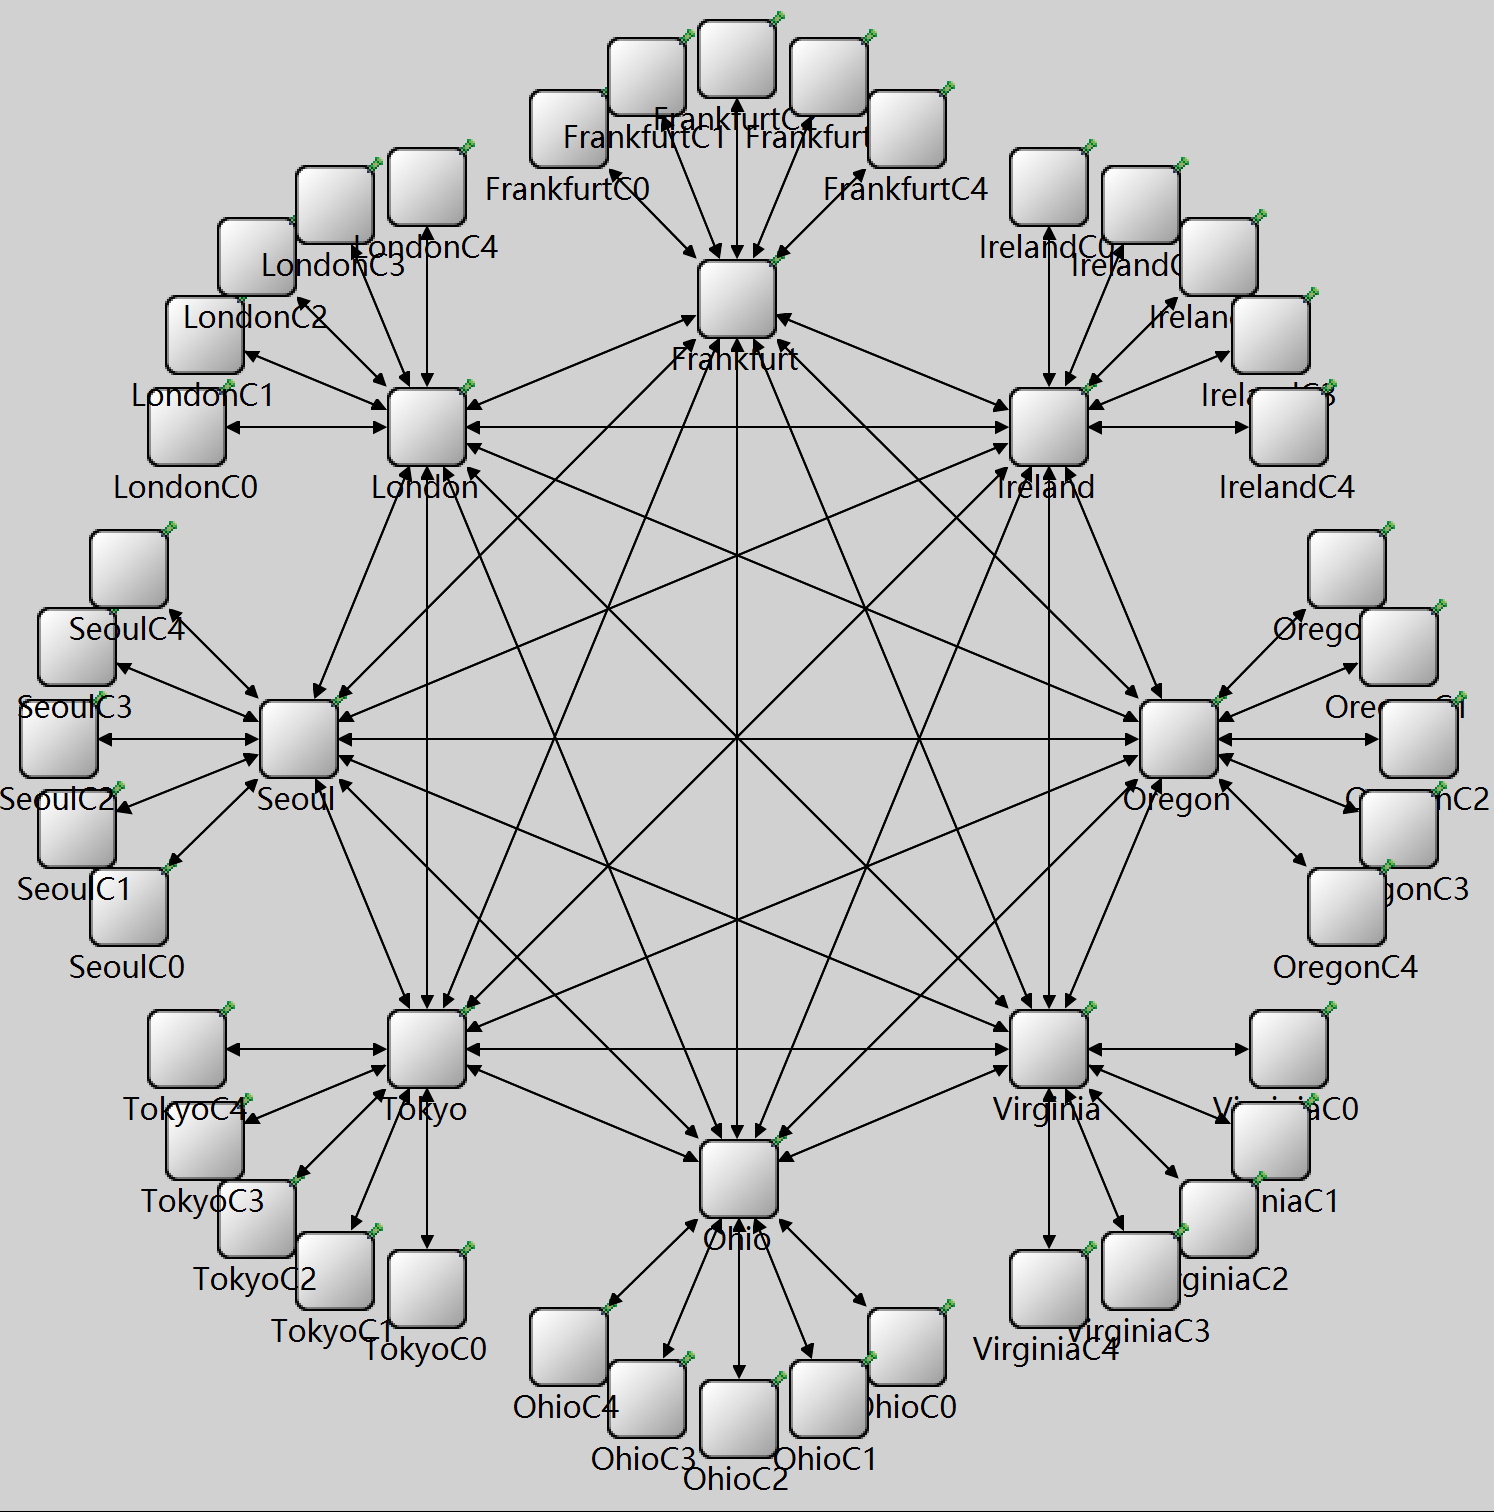
\includegraphics[width=0.4\linewidth]{fig/our_topology.png}
    \end{figure}
    \begin{itemize}
        \item Simulation based on C++
        \item Considering latency, bandwidth, and computation resources
    \end{itemize}
\end{frame}

\begin{frame}{Result}
    Setup:

    \vspace{0.5em}
    \begin{center}
    \small
    \begin{tabular}{l|l}
        \textbf{Parameter} & \textbf{Value} \\
        \hline
        $\mathbb N$ (\# input tokens) & $10^9$ \\
        \hline
        $\mathbb B$ (batch size) & $10^6$ \\
        \hline
        $n$ (\# clusters) & 8 \\
        \hline
        $m_i$ (\# clients in clusters) & 5 \\
        \hline
        $c_{i,j}$ (compute FLOPS) & $\approx 10^{14}$ \\
        \hline
        $v_{i, j}, w_{i, j} $ (intra' latency, bandwidth) & (median consumer link in country)  \\
        \hline
        $V_{i, j}, W_{i, j}$ (inter' latency, bandwidth) & (AWS instance benchmark)
    \end{tabular}
    \end{center}

    Result:

    \vspace{0.5em}
    \begin{center}
    \small
    \begin{tabular}{l|l}
        \textbf{$B$ (microbatch size)} & \textbf{Time to train (days)} \\
        \hline
        $100,000$ & $581.36$ \\
        \hline
        $50,000$ & $476.70$ \\
        \hline
        $10,000$ & $452.70$
    \end{tabular}
    \end{center}
\end{frame}

\begin{frame}{The End}
\huge{\centerline{Thank you for listening!}}

\vspace{1cm}
\normalsize
\end{frame}

\end{document}
